
Para extender esta noci\'on de integral a  conjuntos acotados m\'as generales que no sean  rect\'angulos, definimos lo siguiente. 

\begin{definition}\label{def:int_D}
Sean $D  \subseteq  \mathbb{R}^{2}$,  $f:D \to\R$ contínua y $R=[a,b]\times[c,d]$ tal que $D  \subseteq  R$.  Se define la funci\'on $f^*$ tal que 
\[
    f^*(x,y)=
    \begin{dcases*}
        f(x,y) & si $(x,y)\in D$ \\[.2cm]
        0        & si $(x,y)\in R \setminus D.$
    \end{dcases*}
\]

Dada su definici\'on, $f^*$ no tiene porque ser continua sobre todo $R$ pero de tener discontinuidades  las mismas estar\'an sobre  $\partial D$. Luego, si $\partial D$ est\'a formada por una curva continua entonces $f^*$ es integrable y  se define la integral de $f$ sobre $D$ por
\[
    \iint_D f\:dA=\iint_B f^*\:dA.  
\]
\end{definition}
La explicación se puede observar mejor en la siguiente figura:


 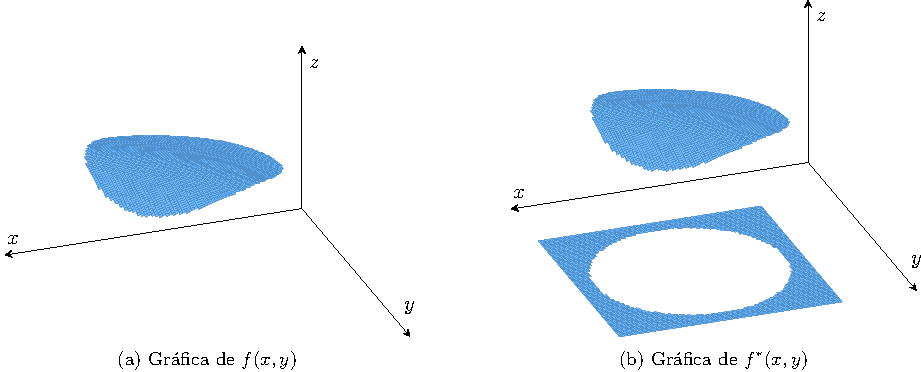
\includegraphics{standalone_fig_integral.pdf}

%\begin{figure}[H]
 %   \centering
 % === Subfigura (a) ===
 %   \begin{subfigure}[b]{0.45\textwidth}
 %   \centering
  %  \begin{tikzpicture}
  %  \begin{axis}[
    %    view={160}{40},
     %   xmin=0, xmax=2,
   %     ymin=0, ymax=2,
    %    zmin=0, zmax=3,
     %   axis lines=center,
     %   ticks=none,
     %   xlabel={$x$}, ylabel={$y$}, zlabel={$z$},
     %   domain=0:2, y domain=0:2,
     %   samples=30, z buffer=sort
  %  ]
        % Región R (rectángulo base)
     %   \addplot3[
    % surf,
  %  shader=faceted,
  %  draw=black, % dibuja las líneas de la malla
   % fill=gray, fill opacity=0.2,
  %  domain=0.5:2, y domain=0.5:2,
  %  samples=20
%] {0};

    %    % Superficie sobre región R (solo en R)
     %   \addplot3[
      %      surf, opacity=0.7, colormap={mycolor}{rgb255=(100,180,255) rgb255=(100,180,255)},
        %    domain=0.5:2, y domain=0.5:2,
      %  ] {sin(x*y*50)+2};
   % \end{axis}
   % \end{tikzpicture}
    % \caption{Gráfica de \( f(x,y) \) sobre  \( R \)}
    % \end{subfigure}
    % \hfill
    % === Subfigura (b) ===
    % \begin{subfigure}[b]{0.45\textwidth}
   % \centering
   % \begin{tikzpicture}
   % \begin{axis}[
     %   view={160}{40},
     %   xmin=0, xmax=2,
     %   ymin=0, ymax=2,
     %   zmin=0, zmax=3,
     %   axis lines=center,
      %  ticks=none,
      %  xlabel={$x$}, ylabel={$y$}, zlabel={$z$},
       %  domain=0:2, y domain=0:2,
      %  samples=60, z buffer=sort
   % ]

     %   % Superficie f(x,y) sobre toda R, con 0 fuera de D
     %   \addplot3[
       %     surf, opacity=0.8,
      %      domain=0.5:1.5, y domain=0.5:1.5,
       %     colormap={mycolor}{rgb255=(100,180,255) rgb255=(100,180,255)},
        %     restrict z to domain=2.1:10, % recorta para evitar planicies
   % unbounded coords=jump,
    %    ]
      %  { ( (x-1)^2 + (y-1)^2 < 0.2 ) * sin(x*y*50)+2 };

         % Región R en gris claro
     % \addplot3[
   % surf,
  %  shader=faceted,
   % draw=black, % dibuja las líneas de la malla
   % fill=gray, fill opacity=0.2,
   % domain=0.5:2, y domain=0.5:2,
  %  samples=20
%] {0};
        
       % \addplot3[
        %    surf, opacity=0.8,
         %   domain=0.5:2, y domain=0.5:2,
        %    colormap={mycolor}{rgb255=(100,180,255) rgb255=(100,180,255)},
      %       restrict z to domain=-0.1:0.1, % recorta para evitar planicies
  %  unbounded coords=jump,
      %  ]
      %  { ( (x-1)^2 + (y-1)^2 < 0.2 ) + 0 };

  %  \end{axis}
   % \end{tikzpicture}
  %  \caption{Gráfica de \( f^*(x,y) \) sobre \( R \)}
  %  \end{subfigure}
%\end{figure}

























\begin{obs} 
La  \autoref{def:int_D}  es independiente  de la selecci\'on de $B$.
\end{obs}

\begin{propertie}
    Sean $f,\;g$ dos funciones integrables en una regi\'on $D\subset\Rn{2}$, entonces:
    \begin{enumerate}
        \item[i.] $\alpha f+\beta g$ es integrable en $D$, $\forall\;\alpha,\;\beta\in\R$ y, adem\'as,
        \[
            \iint_D \left(\alpha f+\beta g\right)dA=\alpha\iint_D f\:dA+\beta\iint_D g\:dA.
        \]
        \item[ii.] El producto $fg$ es integrable en $D$.
        \item[iii.] Si $g(x,y) \neq 0\;\forall(x,y)\in D$ entonces el cociente $f/g$ es integrable en $D$.
        \item[iv.] Si $f(x,y)\geq 0 \;\forall(x,y)\in D$ entonces  $\iint_D f\:dA\geq0$.
        \item[v.]Si $f(x,y)\leq g(x,y)  \;\forall(x,y)\in D$ entonces $\iint_D f\:dA\leq\iint_D g\:dA.$
        \item[vi.]Si $|f|$ es integrable en $D$ entonces 
        \[
            \left|\iint_D f\:dA\right|\leq\iint_D|f|\:dA.  
        \]    
        \item[vii.] Si $D=D_1\cup D_2$ donde $\;D_1\cap D_2$ es un conjunto de medida nula  entonces   $f$ es integrable sobre $D_1$ y sobre $D_2$ y, adem\'as,  
        \[
            \iint_D f\:dA=\iint_{D_1} f\:dA+\iint_{D_2}f\:dA.    
        \]
    \end{enumerate}
\end{propertie}
